\documentclass[border=6pt]{standalone}
\usepackage{lmodern}
\usepackage{tikz}
\usetikzlibrary{arrows.meta,positioning,calc}

\begin{document}
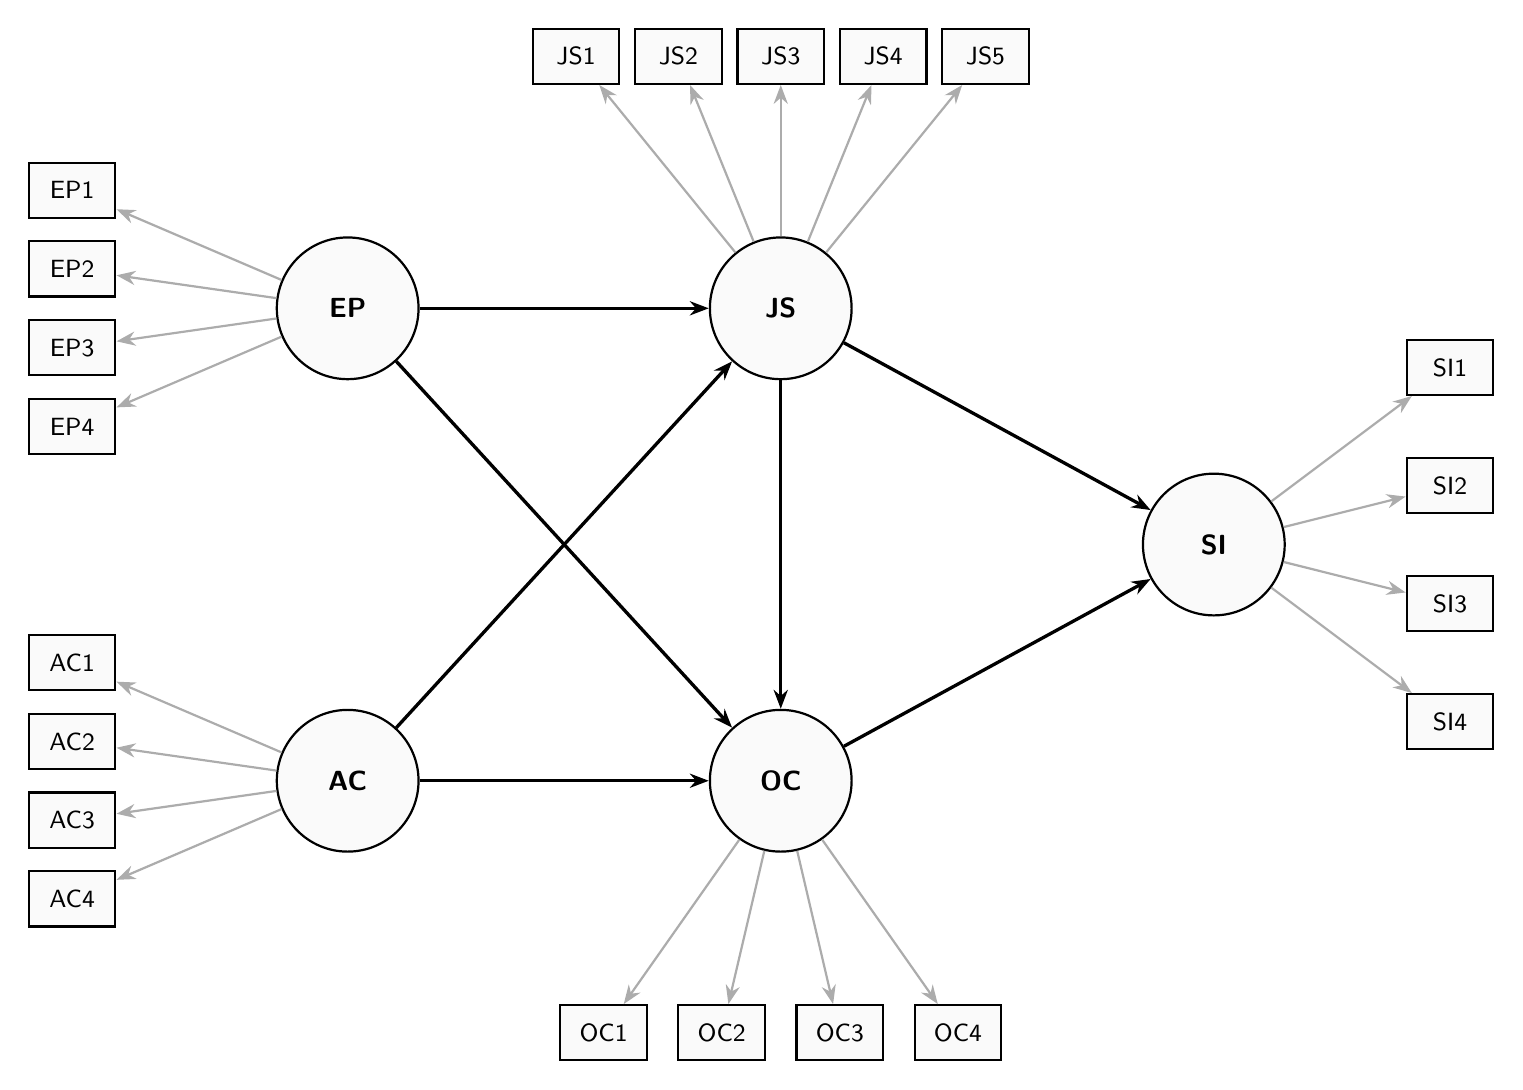
\begin{tikzpicture}[
  >={Stealth[length=2.4mm]},
  font=\sffamily,
  construct/.style={circle, draw, thick, minimum size=18mm, align=center,
                    inner sep=0pt, fill=gray!4},
  indicator/.style={rectangle, draw, thick, minimum width=11mm,
                    minimum height=7mm, fill=gray!4, font=\small\sffamily},
  load/.style={->, thick, gray!65},
  path/.style={->, very thick, black},
  loadlab/.style={font=\scriptsize, inner sep=1pt, fill=white, text=black!75},
  pathlab/.style={font=\small\bfseries, inner sep=1.5pt, fill=white}
]
\newcommand{\rsq}[1]{\\[1pt]{\scriptsize\itshape #1}}

% ---------- Constructs ----------
\node[construct] (EP) at (0,3)    {\textbf{EP}};
\node[construct] (AC) at (0,-3)   {\textbf{AC}};
\node[construct] (JS) at (5.5,3)  {\textbf{JS}};
\node[construct] (OC) at (5.5,-3) {\textbf{OC}};
\node[construct] (SI) at (11,0)   {\textbf{SI}};

% ---------- Indicators ----------
% EP (left, top block)
\foreach \i/\y in {1/4.5,2/3.5,3/2.5,4/1.5}
  \node[indicator] (EP\i) at (-3.5,\y) {EP\i};
% AC (left, bottom block)
\foreach \i/\y in {1/-1.5,2/-2.5,3/-3.5,4/-4.5}
  \node[indicator] (AC\i) at (-3.5,\y) {AC\i};
% JS (top)
\foreach \i/\x in {1/2.9,2/4.2,3/5.5,4/6.8,5/8.1}
  \node[indicator] (JS\i) at (\x,6.2) {JS\i};
% OC (bottom)
\foreach \i/\x in {1/3.25,2/4.75,3/6.25,4/7.75}
  \node[indicator] (OC\i) at (\x,-6.2) {OC\i};
% SI (right)
\foreach \i/\y in {1/2.25,2/0.75,3/-0.75,4/-2.25}
  \node[indicator] (SI\i) at (14,\y) {SI\i};

% ---------- Measurement (reflective) ----------
\foreach \i in {1,2,3,4} \draw[load] (EP) -- (EP\i);
\foreach \i in {1,2,3,4} \draw[load] (AC) -- (AC\i);
\foreach \i in {1,2,3,4,5} \draw[load] (JS) -- (JS\i);
\foreach \i in {1,2,3,4} \draw[load] (OC) -- (OC\i);
\foreach \i in {1,2,3,4} \draw[load] (SI) -- (SI\i);

% ---------- Structural (paths) ----------
\draw[path] (EP) -- (JS);
\draw[path] (EP) -- (OC);
\draw[path] (AC) -- (JS);
\draw[path] (AC) -- (OC);
\draw[path] (JS) -- (OC);
\draw[path] (JS) -- (SI);
\draw[path] (OC) -- (SI);

\end{tikzpicture}
\end{document}
